\documentclass[10pt,twocolumn,twoside,lineno]{gsajnl}
% Use the documentclass option 'lineno' to view line numbers

\usepackage{epstopdf}

\usepackage{float} % Stop tables from floating

\articletype{inv} % article type
% {inv} Investigation
% {gs} Genomic Selection
% {goi} Genetics of Immunity
% {gos} Genetics of Sex
% {mp} Multiparental Populations

\runningtitle{Unveiling the Role of Competition Mechanism in the Progression of Cancer} % For use in the footer
\runningauthor{Ajoku \textit{et al.}}

\title{Unveiling the Role of Competition Mechanism in the Progression of Cancer}

\author[$\dagger$]{Chukwudi Ajoku}
\author[$\dagger$]{Lauren McGinney}
\author[$\dagger$]{Claudio Angione}
\author[$\ast$]{Pietro Li\`{o}}
%\author[2,3]{Author Four}
\author[$\dagger$]{Alessandro Di Stefano}
\author[$\dagger$]{Annalisa Occhipinti}

\affil[$\dagger$]{Teesside University}
\affil[$\ast$]{University of Cambridge}

% Use the \equalcontrib command to mark authors with equal
% contributions, using the relevant superscript numbers
%\equalcontrib{1}
%\equalcontrib{2}

%\correspondingauthoraffiliation[$\ast$]{Corresponding author: Please insert the affiliation correspondence address and email for the corresponding author. The corresponding author should be marked with the relevant number in the author list, as shown in the example.}

\begin{abstract}
The abstract should be written for people who may not read the entire paper, so it must stand on its own. The impression it makes usually determines whether the reader will go on to read the article, so the abstract must be engaging, clear, and concise. In addition, the abstract may be the only part of the article that is indexed in databases, so it must accurately reflect the content of the article. A well-written abstract is the  most effective way to reach intended readers, leading to more robust search, retrieval, and usage of the article.

Please see additional guidelines notes on preparing your abstract below.
\end{abstract}

\keywords{Multi-omics Data; Interpretable Deep Learning; Cancer Metabolism; Survival Analysis}

\dates{\rec{xx xx, xxxx} \acc{xx xx, xxxx}}

\begin{document}

\maketitle
\thispagestyle{firststyle}
%\slugnote
%\firstpagefootnote
\vspace{-13pt}% Only used for adjusting extra space in the left column of the first page

\lettrine[lines=2]{\color{color2}T}{}he use of Artificial Neural Networks can be a great advantage in the prediction of patients survival using clinical and genomic data. One downside to this is the multidimensionality of genomic datasets which usually spans thousands of columns. For Machine Learning to work effectively, it is important that there are more sampled observations than there are variables/features. One rule of thumb for classification models is to have at least 10 times as many rows as you have columns and for regression models, at least 50 times as many rows as the number of columns should be sufficient \citep{googledoc}. For this reason, working with genomic datasets has proven to be difficult due to the lack of sufficient samples (which should run into hundreds of thousands) 


To solve this problem, this paper introduces a technique, a feature selection strategy which reduces the number of required features. In this technique, using a patients gene expression data, the active reactions and pathways in a patient is derived and used instead of the genes themselves. \verb|(More justification needed)|.


\section{Background}
The complex molecular processes behind cancer patient survival can be understood using genetic and clinical data, not only to create novel therapies for patients, but also to enhance survival prediction \citep{doi:10.4137/BIC.S33380}. Due to the effective generation of high-dimensional genomic data (e.g., gene expression data and RNA-seq) by modern molecular high-throughput sequencing techniques, molecular profiles of human illnesses (e.g., cancer) may be generated \citep{10.1093/bib/bby051}. High-dimensional biological data are increasingly being used to both elucidate the underlying biological processes of disease and to aid in therapeutic decision making.



Survival analysis is a collection of techniques for estimating the survival distribution from data, with the result being the time required for an observation to experience an event of interest. It is critical in survival analysis to properly handle censoring data, which are another kind of missing value. The Cox Proportional Hazards regression model (Cox-PH) is the most often used method for analysing time-to-event data in clinical trials \citep{Ahmed2007, Chen2012}. It is a semi-parametric model with minimal assumptions that is good at interpreting the impact of risk variables on one another. For example, almost 15,000 patients with breast cancer were analysed using both standard and stratified Cox models to determine the relationship between cancer therapies and survival time, as well as cancer stage \citep{Abadi2014}. Additionally, a Cox-PH model was used to determine the effect of chronic illnesses on cancer patient survival in about 400 breast cancer patients \citep{Atashgar}.



However, the primary limitations of the traditional Cox-PH model are (1) the inability to analyse data with a large number of dimensions and a small sample size (HDLSS); and (2) the inability to handle highly nonlinear relationships between variables. Analyzing HDLSS data is critical and difficult in bioinformatics, since the majority of biological data contain a small number of samples ($n$) but a high number of characteristics ($p$), i.e., $p > n$. High-dimensional data often result in either training being impossible or the training dataset being overfit \citep{Witten2009}. As a result, data with a low dimension and a high sample size, such as clinical data, are utilised to directly apply the conventional Cox-PH model for predicting patient survival outcomes.

Nonetheless, there has been a significant increase in research using the analysis of high-dimensional genomic data in order to ascertain the impact of the molecular biological process on patient survival.
In general, techniques for feature selection, such as penalization algorithms, have been explored to solve the HDLSS problem in the Cox-PH model.
For high-dimensional genomic data, penalty-based Cox-PH models with LASSO (L 1 ) or elastic-net regularisation were widely employed \citep{10.1093/biomet/asm037, Tibshirani+2009, JSSv039i05, Xu2012}.
Additionally, an improved feature selection strategy was suggested to ensure that the selection process took into account almost all important variables \citep{Fan2010}.



Although the impact of genetic data on patient survival are typically extremely nonlinear for complicated human illnesses \citep{MALLAVARAPU202024}, the traditional Cox-PH model assumes that variables contribute linearly. For linear regression methods, the kernel approach may be used to directly convert nonlinear covariate effects into linear ones. To account for the nonlinear impact of gene expression profiles on censored survival phenotypes such as overall survival time and relapse time, a kernel-based Cox-PH model was suggested \citep{LI2002}. Additionally, two survival support vector machine (SVM) models were suggested to enhance survival prediction using high-dimensional genomic data \citep{10.1093/bioinformatics/btn253}. It is still difficult to find the optimum kernel function with the optimal combination of hyper parameters, since kernel-based models need the kernel function to be specified in advance.



Deep learning methods have lately gained interest in bioinformatics due to their ability to automatically capture nonlinear connections from their input and their ability to build adaptable models. Several deep learning algorithms have been suggested for predicting patient survival that include a conventional Cox-PH model as an output layer. DeepSurv combines a conventional Cox-PH regression with a deep feed-forward neural network to enhance survival prediction and ultimately develop a recommendation system for customised therapy \citep{Katzman2018}. DeepSurv outperforms both conventional Cox-PH and random survival forests (RSFs). However, a drawback of DeepSurv is that it analysed only extremely low-dimension clinical data with fewer than 20 variables. To analyse high-throughput RNA sequencing data, Cox-nnet, an artificial neural network for a regularised Cox-PH regression issue, was suggested \citep{Ching2018}. Cox-nnet beat regularised Cox-PH regression (alone), RSF, and Cox-Boost in the aggregate. Cox-nnet associates patient survival with the top-ranked hidden nodes, which are latent representations of gene expression data, and each hidden node may implicitly reflect a biological activity. Similarly, SurvivalNet used Bayesian Optimization to optimise the structure of a deep neural network automatically \citep{Yousefi2017}. SurvivalNet outperformed Cox elastic net (Cox-EN) and RSF by a little margin. Surprisingly, a properly trained SurvivalNet can calculate the risk score for each node via risk backpropagation analysis.



However, applying deep learning methods to high-dimensional genomic data for survival analysis remains difficult due to the following factors: (1) an overfitting issue when training a deep learning model using HDLSS data; and (2) the absence of clear model interpretation. Models of deep neural networks include a huge number of parameters. As a result, deep learning is usually associated with a high number of samples. Gradients have a large variance in backpropagation when training a deep learning model using HDLSS data, which results in model overfitting. Both Cox-nnet and SurvivalNet used feature selection techniques to incorporate only important genomic data, avoiding the overfitting issue; nevertheless, the methods may struggle with high-dimensional data. To address the HDLSS issue in deep learning, dimension reduction methods were used to decrease the dimension of the input data, and the resulting lower-dimensional data were then fed into a neural network \citep{W2019}. Deep Feature Selection was created to aid in the identification of discriminative features inside a deep learning model \citep{doi:10.1089/cmb.2015.0189}. Deep Neural Pursuit was used to train a small subnetwork and calculate low-variance gradients for feature selection \citep{ijcai2017-318}.



Although deep learning topologies vary, the majority of traditional deep neural networks analyse structural data using many fully connected layers, which makes them challenging to understand. Model interpretation (e.g., identifying prognostic variables) is often more essential in survival analysis than merely predicting patient survival with high accuracy. However, hidden nodes derived from fully linked layers are incapable of representing explicit biological components. Additionally, biological processes may include a subset of biological components rather than all input characteristics. Thus, the capacity of deep neural networks to provide explicit model interpretation is greatly sought in survival analysis.



Additionally, the interpretation of biological pathways' hierarchical interconnections has received little attention. Intuitively, biological interpretation at the route level allows the acquisition of rich biological data. This is because genomic studies have an extraordinary capacity for repeatability. For example, highly repeatable biomarkers for breast cancer diagnosis have been discovered using a high-level representation of metabolic pathway-based characteristics \citep{Huang2016}.



Biological systems are often complicated, and hierarchical interactions between molecular pathways are not uncommon. Disparities in survival rates between patients may be explained by the hierarchical connections across circuits. In particular, the hierarchical representation of receptor pathways and gene ontology was investigated for antiviral signalling \citep{Masson2014}. As a result, by integrating the effects of inhibition and propagation across pathways, a deep learning model may be physiologically interpretable.



It is also difficult to integrate various kinds of data (e.g., multi-omics data or clinical data) into a deep learning model. Numerous research have shown that integrating multi-omics and clinical data enhances survival analysis prediction performance \citep{Yousefi2017, 10.1371/journal.pone.0154313, Zhu2017}. To integrate multi-omics data in a naïve manner, all kinds of data are combined into a single matrix and a survival analysis is performed \citep{Yousefi2017, Zhang2013}. The method is predicated on the assumption that heterogeneous data may be represented using an augmented matrix form. However, the enlarged matrix introduces complications: (1) it produces data with a much greater dimension than HDLSS data; (2) it reduces the sample size owing to missing values; and (3) it disregards data types with fewer variables. Notably, multi-omics data on The Cancer Genome Atlas (TCGA) include significant missing values; for example, 160 mRNA-Seq samples are accessible, while 595 clinical samples are included in the TCGA's glioblastoma multiforme (GBM) dataset.



By combining high-dimensional genomic and clinical data, we create a new pathway-based sparse deep neural network called Cox-PASNet for survival analysis.
Our primary contributions to survival analysis with Cox-PASNet are: 
\begin{itemize}
	\item identifying nonlinear and hierarchical relationships at the biological gene and pathway levels;
	\item providing a solution for neural network model interpretation in which each node represents a biological component or process;
	\item integrating multiple types of data in a deep learning model; and
	\item proposing efficient optimization for survival analysis.
\end{itemize}

This article is an expanded version of a paper titled Cox-PASNet: Pathway-based Sparse Deep Neural Network for Survival Analysis, which was presented at the IEEE International Conference on Bioinformatics and Biomedicine (IEEE BIBM 2018), which took place in Madrid, Spain, from December 3 to 6, 2018 \citep{8621345}. 


\section{Results}
\subsection{Datasets}

We evaluated the efficacy of Cox-PASNet, the suggested model, on glioblastoma multiforme (GBM) and ovarian serous cystadenocarcinoma (OV) tumours in this research. GBM is the most aggressive kind of malignant tumour, growing quickly inside the brain and with a bad prognosis \citep{no28}; OV cancer is the most prevalent type of cancer in women worldwide, and it is often detected at a late stage \citep{BrettM2017}. cBioPortal (www.cbioportal.org/datasets) was used to get gene expression and clinical data for TCGA GBM and OV malignancies. We eliminated patients who did not have a survival time or an event status.


We acquired biological pathways as previous information from the Molecular Signatures Database (MSigDB) \citep{Subramanian15545}, where we analysed pathways using both the KEGG and Reactome databases. We excluded small pathways (those containing fewer than fifteen genes) and large pathways (those containing more than 300 genes), as small pathways are frequently redundant with other larger pathways and large pathways are associated with more general biological pathways rather than disease-specific pathways \citep{Reimand2019}. Additionally, we looked at the genes that were associated with at least one of these pathways.


Additionally, we included clinical data from individuals with GBM and OV cancer. Only age was included in the clinical layer of Cox-PASNet, since age was a significant prognostic factor in GBM \citep{10.1371/journal.pone.0154313}, and the majority of other clinical information was absent. For example, in addition to age, the Karnofsky Performance Score (KPS) has been identified as a major determinant. However, there is a significant connection between KPS and age, and many patients do not have access to their KPS data. Finally, we have data on 5,404 genes, 659 pathways, and clinical ages from 523 patients with GBM and 532 individuals with OV cancer.

\subsection{Experimental design}

Cox-prediction PASNet's performance was assessed in comparison to state-of-the-art techniques such as Cox-EN \citep{JSSv039i05}, Cox-nnet \citep{Ching2018}, and SurvivalNet \citep{Yousefi2017}. We used the C-index to assess predictive performance using censored data. This is a rank correlation technique that counts concordant pairings between the predicted score and observed survival time. The C-index ranges between 0 and 1, with 1 indicating a perfect forecast and 0.5 indicating a random guess.


We performed the holdout assessment 20 times to ensure model performance was reproducible, given the limited sample size, with the two goals of survival months and censor status (i.e., alive or dead), as well as computing costs. Each experiment used a random sample of 20\% of the dataset for test data and the remaining 80\% for training data (80\% ) and validation data (20\% ), while guaranteeing the same censoring percentage on training, validation, and test data. We normalised the gene expressions and ages in the training data to a zero mean and unit standard deviation. Then, we normalised the validation and test data using the corresponding mean and standard deviation values derived from the training data, such that no information from the test data was utilised for training. The training data were used to train each model, and the validation data were used to determine the optimum pair of hyperparameters. Once the model was well-trained, the prediction performance was evaluated using test data.

\subsection{Model tuning}

Cox-PASNet was developed using current deep learning model. We chose the Tanh function as the activation function since it provided the greatest C-index score when compared to ReLU and LeakyReLU. Additionally, Tanh is advantageous since it offers a probabilistic meaning for the activation of a node. We examined both dropout and $ L^{2} $ regularisation. Dropout rates were empirically determined to be 0.7 and 0.5 in the route layer and the first hidden layer, respectively. Adaptive Moment Estimation (Adam) was used to improve the neural network \citep{kingma2017adam}, where a grid search was used to estimate the optimum learning rate ($ \eta $) and $ L^{2} $ penalty term ($ \lambda $). On each trial, the optimum hyper-parameters of $ \eta $ and $ \lambda $ were selected in order to minimise the cost function using validation data, and the model was then trained using the optimal hyper-parameters. Cox-PASNet is publicly accessible in the PyTorch framework at \url{https://github.com/DataX-JieHao/Cox-PASNet.}


To provide a roughly equal comparison, we used the Python programme Glm-net Vignette \citep{JSSv039i05} for the Cox-EN model. The optimum hyperparameters $ \alpha $ and $ \lambda $ of and were determined via a grid search, similar to what Cox-PASNet accomplished. Candidates for $ \alpha $ are in the range [ 0, 1], with a stride length of 0.01 and $ \lambda $ length of 200. Then, using the training data, we trained the Cox-EN model with the optimum hyperparameters and assessed the model's performance using the related test data. Cox-nnet was trained using the implementation codes available on the authors' GitHub repository. For $ L^{2} $, we utilised the default tuning setting and ran a grid search. With regards to SurvivalNet, we improved the hyperparameters using the Bayesian Optimization method, BayesOpt, which was recognised for its ability to optimise the SurvivalNet automatically \citep{DBLP:journals/corr/Martinez-Cantin14}. Apart from their default search, we introduced two more hyper-parameters to the BayesOpt algorithm: $ L^{1} $ and $ L^{2} $ penalty terms. SurvivalNet was built using open source code available on the authors' GitHub.


To integrate two distinct kinds of data, we combined gene expression and clinical age data into a large input matrix and fed it into benchmark models like as Cox-EN, Cox-nnet, and SurvivalNet. Meanwhile, we independently added data on gene expression and clinical age to the gene and clinical layers.



\subsection{Experimental results}

Fig. 1 and Tables 1 and 2 illustrate the experimental findings using GBM and OV cancer data. With GBM data, our suggested Cox-PASNet has the highest C-index (0.63470.0372), followed by Cox-nnet (0.59030.0372). (see Fig. 1a and Table 1). Cox-nnet is a kind of artificial neural network with a single hidden layer. SurvivalNet is a multilayer perceptron, which is a more sophisticated model than Cox-nnet, and the BayesOpt algorithm determines the optimum design of SurvivalNet. Meanwhile, Cox-nnet demonstrated that a smaller neural network often outperforms a deeper network [17]. As a result, SurvivalNet generated an average C-index of 0.55210.0295 that was less than Cox- nnet's. Additionally, Cox-EN produced a C-index of 0.51510.0336 that was almost identical to a random estimate. Cox-suboptimal EN's performance may be explained by the extremely nonlinear nature of biological data, which include 5,404 gene expressions but only 523 patients. A Wilcoxon test was used to determine if the outperformance of Cox-PASNet over the other three benchmarks was statistically significant. Table 3 clearly shown that Cox-PASNet outperformed Cox-EN, Cox-nnet, and SurvivalNet, respectively.



Additionally, we assessed Cox-PASNet using OV cancer data. Additionally, Cox-PASNet achieved the highest C-index of 0.63430.0439; Cox-nnet maintained the second position with a C-index of 0.60950.0356; and Cox-EN took the last position with a C-index of 0.52760.0482. (Fig. 1b and Table 2). In Table 4, the Wilcoxon test revealed that Cox-PASNet also outperformed others statistically in OV cancer.

\begin{figure}
	content...
\end{figure}

It is worth noting that Cox-PASNet employs the same loss function as Cox-EN, Cox-nnet, and SurvivalNet, which is a negative log partial likelihood. Nonetheless, in Cox-PASNet, we combine a deep neural network design with previous biological information about routes. The biologically motivated neural network performs better in terms of prediction and minimises noisy signals generated by complicated biological input. Additionally, to avoid overfitting, Cox-PASNet was trained using tiny sub-networks. Thus, Cox-PASNet provides two contributions to prediction performance: the biologically driven design and the novel training method.



\begin{table}[H]

	\caption{Comparison of C-index with GBM in over 20 experiments}
	\begin{tableminipage}{0.482\textwidth}
		\begin{tabularx}{\textwidth}{@{}XX@{}}
			\hline
			{\bf Model} & {\bf C-index}\\
			\hline
			Cox-EN & $ 0.5151 \pm 0.0336 $ \\
			Cox-nnet & $ 0.5903 \pm 0.0372 $ \\
			SurvivalNet & $ 0.5521 \pm 0.0295 $ \\
			Cox-PASNet & $ 0.6347 \pm 0.0372 $ \\
			\hline
		\end{tabularx}
		\label{tab:shape-functions}
	\end{tableminipage}
\end{table}


\begin{table}[H]
	
	\caption{Comparison of C-index with OV cancer in over 20 experiments}
	\begin{tableminipage}{0.482\textwidth}
		\begin{tabularx}{\textwidth}{@{}XX@{}}
			\hline
			{\bf Model} & {\bf C-index}\\
			\hline
			Cox-EN & $ 0.5276 \pm 0.0482 $ \\
			Cox-nnet & $ 0.6095 \pm 0.0356 $ \\
			SurvivalNet & $ 0.5614 \pm 0.0524 $ \\
			Cox-PASNet & $ \mathbf{0.6343 \pm 0.0439} $ \\
			\hline
		\end{tabularx}
		\label{tab:shape-functions}
	\end{tableminipage}
	\footnotesize{Bolded indicates the highest performance.}
\end{table}



\section{Discussion}
\subsection{Model Interpretation}


We re-trained Cox-PASNet using the best pair of hyper-parameters from 20 trials utilising all available GBM data to understand the biological model.
The median Prognostic Index (PI), which is the output value of Cox-PASNet, was used to classify the samples into two groups: high-risk and low-risk.
Figs. 2 and 3 show the node values for the two groups in the integrative layer (i.e., the second hidden layer (H2) and the clinical layer) and the route layer, respectively.
The node values of 31 variables (30 from genomic data and age from clinical data) were sorted according to their average absolute partial derivatives with respect to the integrative layer in Fig. 2a.
In terms of partial derivatives, age (the first column in Fig. 2a) is revealed to be the most significant covariate in Cox-PASNet using GBM data.



The top-ranked variables had significantly different distributions in high- and low-risk groups.
For example, in the high-risk group, the first three variables in H2 (the second, third, and fourth columns in Fig. 2a) were active, but were deactivated in the low-risk group.
Additionally, we conducted a logrank test by dividing the covariate's node values into two groups based on their medians.
The logrank test's -log10(p-values) output is shown in the top panel, aligned with the variables in Fig. 2a.
Significant variables are shown by red triangles (-log10(p-value) >1.3), while inconsequential covariates are indicated by blue triangles.
The logrank tests showed that the variables with the highest absolute weight are predictive of survival.
Kaplan-Meier curves for the top two variables are shown in Figure 2b-c, indicating that survival rates between the two groups are substantially different.
As a result, the top-ranking covariates may be termed prognostic variables. 


\begin{table}[H]
	
	\caption{Statistical assessment with GBM}
	\begin{tableminipage}{0.482\textwidth}
		\begin{tabularx}{\textwidth}{@{}XX@{}}
			\hline
			 & {\bf Wilcoxon rank-sum test}\\
			\hline
			Cox-PASNet vs. Cox-EN & $ 8.85e-05 ^{*} $ \\
			Cox-PASNet vs. Cox-nnet & $ 4.49e-4 ^{*} $ \\
			Cox-PASNet vs. SurvivalNet & $ 1.40e-4 ^{*} $ \\
			\hline
		\end{tabularx}
		\label{tab:shape-functions}
	\end{tableminipage}
	\footnotesize{$ ^{*} $ shows the statistical significance with significance level = 0.05}
\end{table}



\begin{table}[H]
	
	\caption{Statistical assessment with OV cancer}
	\begin{tableminipage}{0.482\textwidth}
		\begin{tabularx}{\textwidth}{@{}XX@{}}
			\hline
			& {\bf Wilcoxon rank-sum test}\\
			\hline
			Cox-PASNet vs. Cox-EN & $ 1.03e-4 ^{*} $ \\
			Cox-PASNet vs. Cox-nnet & $ 0.04 ^{*} $ \\
			Cox-PASNet vs. SurvivalNet & $ 2.93e-4 ^{*} $ \\
			\hline
		\end{tabularx}
		\label{tab:shape-functions}
	\end{tableminipage}
	\footnotesize{$ ^{*} $ shows the statistical significance with significance level = 0.05}
\end{table}


Similarly, Fig. 3 illustrates the nodes in the route layer in part. The heatmap in Fig. 3a shows the top ten pathway node values for the high-risk and low-risk groups, where the pathway nodes are ordered according to their average absolute partial derivatives with respect to the route layer. Additionally, we conducted logrank tests on each route node, and the survival analysis revealed that 304 out of 659 pathways were statistically significant. A Kaplan-Meier analysis was performed on the two top-ranked routes, as illustrated in Fig. 3b-c. The Kaplan-Meier curves for the two top-ranked routes indicate that the pathway nodes have the potential to serve as prognostic variables.



The integrative layer's statistically significant nodes and the top ten ranked route nodes are shown in Fig. 4 using t-SNE [34]. The diagram illustrates the nonlinearity of the nodes related with PI. The integrative layer represents hierarchical and nonlinear route combinations. As a result of this, the more distinct connections

The integrative layer has more survivals than the route layer.

The top 10 routes, together with their associated literature, are presented in Table 5. The logrank test was used to calculate the p-values in the table using the route node values for the two groups of high and low risks. Five of these routes have been identified as important in the biology literature regarding GBM. The Jak-STAT signalling system, which is often referred to as an oncopathway, is activated in a variety of human malignancies to promote tumour development [35]. By inhibiting the Jak-STAT signalling system, malignant tumours may be reduced in animal models of glioma. One of the most important routes in GBM has been identified as a neuroactive ligand-receptor interaction [38]. The PI3K cascade is another well-known route that plays a significant role in the proliferation, invasion, and migration of GBM cells [39].

\begin{figure}
	content...
\end{figure}


\begin{figure}
	content...
\end{figure}


The top 10 genes, as determined by partial derivatives with respect to each gene, are presented in Table 6 along with their p-values and relevant literature. Because PRL expression has been linked to the development of neoplasms and central nervous system neoplasms, an evaluation of PRL expression in primary central nervous system malignancies was conducted [42]. MAPK9, along with RRM2 and XIAP, has been discovered as a new potential therapeutic marker linked with the molecular processes implicated in the carcinogenesis of GBM [43]. IL22 has been shown to induce the malignant transformation of bone marrow-derived mesenchymal stem cells, which have strong tumoritropic migratory characteristics and are used in tumour therapy [44]. FGF5 acts as an oncogenic factor in human astrocytic brain tumours, contributing to their malignant development [45]. JUN activation, in conjunction with HDAC3 and CEBPB deregulation, seems to provide resistance on hypoxia GBM cells to chemotherapy and radiation treatment; while downregulation of the genes appeared to limit temozolomide action on hypoxic GBM cells [46]. Low DRD5 expression was linked with significantly better clinical outcomes in glioblastoma patients with ONC201 [47]. HTR7 has been implicated in the formation and progression of diffuse intrinsic pontine glioma [48]. It is engaged in neuroactive ligand-receptor interaction and the calcium signalling pathway.

\begin{figure}
	content...
\end{figure}


\begin{table*}[t]
	\centering
	\caption{Ten top-ranked pathways in GBM by Cox-PASNet}
	\begin{tableminipage}{\textwidth}
		\begin{tabularx}{\textwidth}{p{350pt}p{50pt}p{50pt}p{50pt}}%{@{}XXXX@{}}
			\hline
			{\bf Pathway name} & {\bf Size} & {\bf P-value} & {\bf Ref.} \\
			\hline
			
			Jak-STAT signaling pathway & 155 & <0.0001 & [35–37] \\
			Neuroactive ligand-receptor interaction & 272 & <0.0001 & [38] \\
			MAP kinase activation in TLR cascade & 50 & 0.0176 & – \\
			NF$\kappa$B and MAP kinases activation mediated by TLR4 signaling repertoire & 72 & 0.0729 & – \\
			G alpha (i) signalling events & 195 & <0.0001 & – \\
			PI3K cascade & 71 & 0.0304 & [39, 40] \\
			Tyrosine metabolism & 42 & 0.5671 & – \\
			Neuronal system & 279 & <0.0001 & [41] \\
			Axon guidance & 129 & 0.0012 & [37] \\
			Xenobiotics & 16 & 0.6347 & – \\
			\hline
		\end{tabularx}
		\label{tab:shape-functions}
	\end{tableminipage}
\end{table*}

It is worth mentioning that only IL22 and FGF5 are statistically significant (i.e., p-value 0.05) by logrank test, implying that only these two genes may be identified as important prognostic variables using standard Cox-PH models. However, additional genes such as PRL, MAPK9, JUN, DRD5, and HTR7 have been scientifically identified as important prognostic factors, despite the absence of substantially distinct gene expression patterns (p-value 0.05). When gene expression changes across genes, the average absolute partial derivatives with respect to each gene quantify the contribution to patient survival made by the pathway and hidden layers in Cox-PASNet. Thus, using Cox-PASNet to identify gene biomarkers enables one to catch important genes that are not linearly linked with patient survival.


Fig. 5 illustrates the Cox-PASNet model's overall interpretation and hierarchical representations at the gene and biological pathway levels. A route node reflects a latent quantity linked with a gene, while a hidden node conveys the high-level representation of a collection of pathways. The subsequent hidden layers reflect the hierarchical representation of the preceding hidden nodes using sparse connections, which aids in identifying critical routes and their interactions that contribute to the system. The final hidden nodes are then put into a Cox-PH model constructed using clinical data.



A pathway node value indicates whether the route is active or inactive, which may be linked with differing survival rates (e.g., Jak-STAT signalling pathway). The relative weight values between the gene layer and the pathway layer may be used to rank the importance of the genes participating in the active pathway (e.g., AKT1). A collection of active routes is represented in the next hidden layer as an active node, which improves survival prediction. For example, the Kaplan-Meier plots of Node 19 and PI in Fig. 5 provide a more comparable estimate of survival than the Jak-STAT signalling pathway.

\subsection{Limitations}
By integrating route databases into the neural network model, Cox-PASNet identifies pathway-based biological processes linked with cancer patient survival. The majority of studies performed post-processed pathway-based analysis on the important genes identified by their models, while Cox-PASNet excluded genes lacking pathway annotations from the study.



We evaluated Cox-PASNet in this research using only GBM and OV tumours from the TCGA. Cross validation using genomic data sets other than TCGA would be useful for further evaluation in future study.
\section{Conclusion}

The potential of deep learning-based survival analysis to uncover nonlinear prognostic variables and its superior prediction performance have been emphasised. However, training deep learning models with high-dimensional data without overfitting and a lack of model interpretability in biology are still unresolved issues. To address these issues, we created a sparse deep neural network based on pathways called Cox-PASNet for survival analysis. Cox-PASNet is a deep learning-based model combined with a Cox proportional-hazards model that can capture nonlinear and hierarchical biological pathway processes and find important prognostic variables related with patient survival. The article introduces a novel model optimization method using HDLSS data for obtaining the optimum sparse model without encountering the overfitting issue. We evaluated Cox-PASNet using TCGA data on GBM and ovarian cancer. The experimental findings demonstrated that Cox-PASNet beat existing cutting-edge survival techniques such as Cox-nnet, SurvivalNet, and Cox-EN, and its predictive performance was evaluated statistically.


Cox-PASNet, like other deep learning-based techniques, considers a negative log-partial likelihood with a single node in the output layer. However, Cox-PASNet builds the neural network on the basis of sparsely coded biological pathways. For model interpretation, genetic and clinical data are incorporated independently into the model.


Cox-PASNet combines both clinical and genomic data. When clinical and genomic data are combined into a big matrix for analysis, the impacts of high-dimensional genomic data may outweigh the effects of clinical data owing to the uneven size of the genomic and clinical variables. Cox-PASNet examines distinct layers for clinical and genomic data, allowing for the interpretation of each data set independently. Additionally, the integration of multi-omics data, such as DNA mutation, copy number variation, DNA methylation, and mRNA expression, is critical for the description of complicated human illnesses, which include a series of complex interactions in many biological processes. As future work, it would also be desired to provide a solution for the integration of complicated heterogeneous data.

\section{Methods}
\subsection{The architecture of Cox-PASNet}
Cox-PASNet is made up of five layers: a gene layer, a pathway layer, numerous hidden layers, a clinical layer, and a Cox layer (see Fig. 6). Cox-PASNet needs two distinct kinds of ordered data: gene expression data and clinical data from the same patient, with gene expression data put into the gene layer and clinical data introduced into the clinical layer. In the final hidden layer, the pipeline layers of the two data types are combined to create a Prognostic Index (PI), which is used as an input to Cox proportional hazards regression. We used age as the only clinical variable in this research. Thus, the clinical layer is immediately integrated inside the final hidden layer, without the need for further hidden layers. Clinical data with a higher dimension is sought to be merged with hidden layers in the clinical process.
\subsubsection{Gene layer}
The gene layer is a Cox-PASNet input layer that combines zero-mean gene expression data (X) with n patient samples expressing p genes, i.e., X = x 1,..., x p and x I N. (0, 1). Only genes that are associated with at least one route are included in the gene layer for pathway-based analysis.

\subsubsection{Pathway layer no  more}
\subsubsection{Hidden layers}
\subsubsection{Clinical layer}
\subsubsection{Cox layer}
\subsubsection{Objective function}
\subsubsection{Sparse coding}


\paragraph{Abbreviations}
\paragraph{Acknowledgements}
\paragraph{About this supplemenr}
\paragraph{Author's contributions}
\paragraph{Funding}
\paragraph{Availability of data and materials}
\paragraph{Ethics approval and consent to participate}
\paragraph{Consent for publication}
\paragraph{Competing interests}
\paragraph{Author details}
\newpage
\paragraph{References}

\bibliography{bibliography}

\subsection{Converted gene expression data(5000+ columns) to active reactions (130+ columns)}
\subsubsection{Used z score normalisation, for any patient, genes with values further away from the mean were considered.}

\section{Discussion}



\section{Guide to using this template in Overleaf}

This template is provided to help you prepare your article for submission to GENETICS.

\section{Author affiliations}

For the authors' names, indicate different affiliations with the symbols: $\ast$, $\dagger$, $\ddagger$, $\S$. After four authors, the symbols double, triple, quadruple, and so forth as required.

\section{Your abstract}

In addition to the guidelines provided in the example abstract above, your abstract should:

\begin{itemize}
\item provide a synopsis of the entire article;
\item begin with the broad context of the study, followed by specific background for the study;
\item describe the purpose, methods and procedures, core findings and results, and conclusions of the study;
\item emphasize new or important aspects of the research;
\item engage the broad readership of GENETICS and be understandable to a diverse audience (avoid using jargon);
\item be a single paragraph of less than 250 words;
\item contain the full name of the organism studied;
\item NOT contain citations or abbreviations.
\end{itemize}

\section{Introduction}

Authors should be mindful of the broad readership of the journal and set the stage for the importance of the work to a generalist reader. The scope and impact of the work should be clearly stated.

In individual organisms where a mutant is being studied, the rationale for the study of that mutant must be clear to a geneticist not studying that particular organism. Similarly, study of particular phenotypes should be justified broadly and not on the basis of interest for that organism alone. General background on the importance of the genetic pathway and/or phenotype should be provided in a single, well-reasoned paragraph near the beginning of the introduction.

\section{Materials and methods}
\label{sec:materials:methods}

Manuscripts submitted to GENETICS should contain a clear description of the experimental design in sufficient detail so that the experimental analysis could be repeated by another scientist. If the level of detail necessary to explain the protocol goes beyond two paragraphs, give a short description in the main body of the paper and prepare a detailed description for supporting information.  For example, details would include indicating how many individuals were used, and if applicable how individuals or groups were combined for analysis. If working with mutants indicate how many independent mutants were isolated. If working with populations indicate how samples were collected and whether they were random with respect to the target population.


\subsection{Statistical analysis}

Indicate what statistical analysis has been performed; not just the name of the software and options selected, but the method and model applied. In the case of many genes being examined simultaneously, or many phenotypes, a multiple comparison correction should be used to control the type I error rate, or a rationale for not applying a correction must be provided. The type of correction applied should be clearly stated. It should also be clear whether the p-values reported are raw, or after correction. Corrected p-values are often appropriate, but raw p-values should be available in the supporting materials so that others may perform their own corrections. In large scale data exploration studies (e.g. genome wide expression studies) a clear and complete description of the replication structure must be provided.

\section{Results and discussion}

The results and discussion should not be repetitive and give a factual presentation of the data with all tables and figures referenced. The discussion should not summarize the results but provide an interpretation of the results, and should clearly delineate between the findings of the particular study and the possible impact of those findings in a larger context. Authors are encouraged to cite recent work relevant to their interpretations. Present and discuss results only once, not in both the Results and Discussion sections. It is acceptable to combine results and discussion in order to be succinct.

\section{Additional guidelines}

\subsection{Numbers} In the text, write out numbers nine or less except as part of a date, a fraction or decimal, a percentage, or a unit of measurement. Use Arabic numbers for those larger than nine, except as the first word of a sentence; however, try to avoid starting a sentence with such a number.

\subsection{Units} Use abbreviations of the customary units of measurement only when they are preceded by a number: "3 min" but "several minutes". Write "percent" as one word, except when used with a number: "several percent" but "75\%." To indicate temperature in centigrade, use ° (for example, 37°); include a letter after the degree symbol only when some other scale is intended (for example, 45°K).

\subsection{Nomenclature and italicization} Italicize names of organisms even when  when the species is not indicated.  Italicize the first three letters of the names of restriction enzyme cleavage sites, as in HindIII. Write the names of strains in roman except when incorporating specific genotypic designations. Italicize genotype names and symbols, including all components of alleles, but not when the name of a gene is the same as the name of an enzyme. Do not use "+" to indicate wild type. Carefully distinguish between genotype (italicized) and phenotype (not italicized) in both the writing and the symbolism.

\subsection{Cross references}
Use the \verb|\nameref| command with the \verb|\label| command to insert cross-references to section headings. For example, a \verb|\label| has been defined in the section \nameref{sec:materials:methods}.

\section{In-text citations}

Add citations using the \verb|\citep{}| command, for example \citep{neher2013genealogies} or for multiple citations, \citep{neher2013genealogies, rodelsperger2014characterization,Falush16}

\section{Examples of article components}
\label{sec:examples}

The sections below show examples of different header levels, which you can use in the primary sections of the manuscript (Results, Discussion, etc.) to organize your content.

\section{First level section header}

Use this level to group two or more closely related headings in a long article.

\subsection{Second level section header}

Second level section text.

\subsubsection{Third level section header:}

Third level section text. These headings may be numbered, but only when the numbers must be cited in the text.

\section{Figures and tables}

Figures and Tables should be labelled and referenced in the standard way using the \verb|\label{}| and \verb|\ref{}| commands.

\subsection{Sample figure}

Figure \ref{fig:spectrum} shows an example figure.

\begin{figure}[t]
\centering
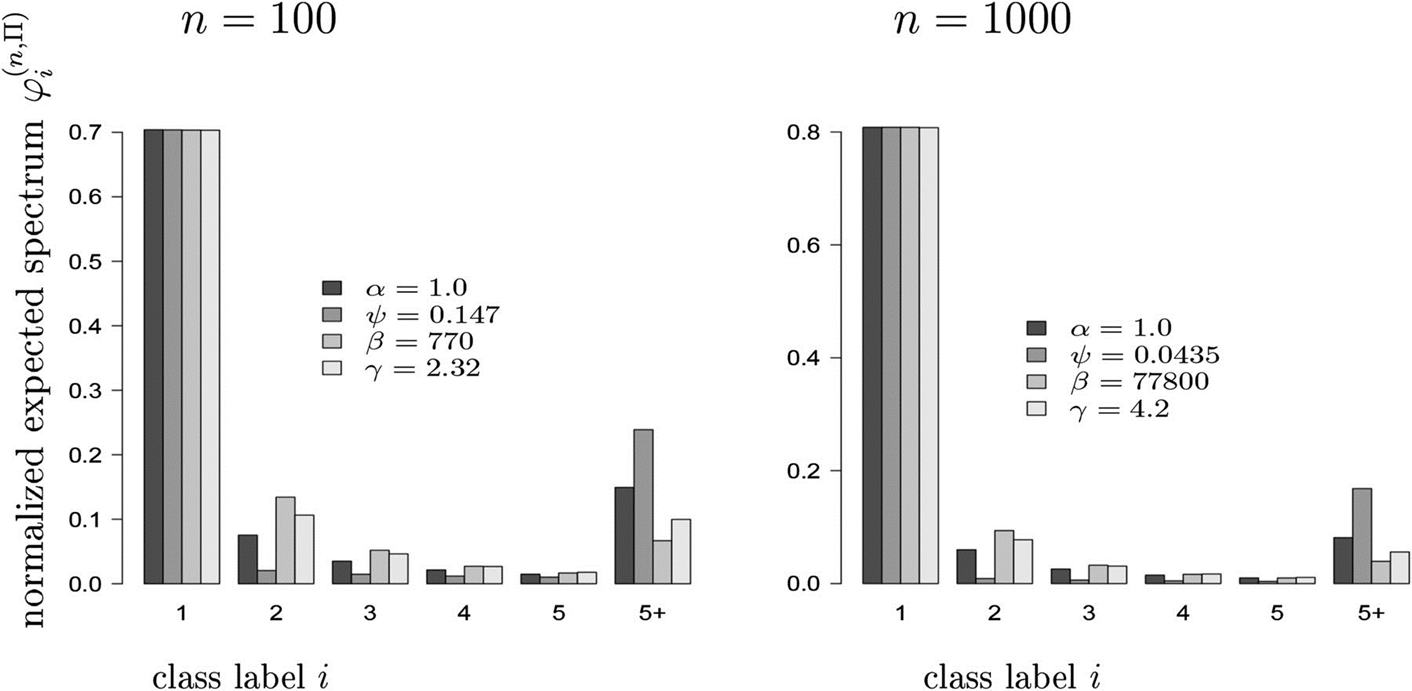
\includegraphics[width=\linewidth]{example-figure}
\caption{Example figure from \url{10.1534/genetics.114.173807}. Please include your figures in the manuscript for the review process. You can upload figures to Overleaf via the Project menu. Images of photographs or paintings can be provided as raster images. Common examples of raster images are .tif/.tiff, .raw, .gif, and .bmp file types. The resolution of raster files is measured by the number of dots or pixels in a given area, referred to as “dpi” or “ppi.”
\begin{itemize}
\item  minimum resolution required for printed images or pictures: 350dpi
\item  minimum resolution for printed line art: 600dpi (complex or finely drawn line art should be 1200dpi)
\item minimum resolution for electronic images (i.e., for on-screen viewing): 72dpi
\protect\end{itemize}
Images of maps, charts, graphs, and diagrams are best rendered digitally as geometric forms called vector graphics. Common file types are .eps, .ai, and .pdf. Vector images use mathematical relationships between points and the lines connecting them to describe an image. These file types do not use pixels; therefore resolution does not apply to vector images.
Label multiple figure parts with A, B, etc. in bolded. Legends should start with a brief title and should be a self-contained description of the content of the figure that provides enough detail to fully understand the data presented. All conventional symbols used to indicate figure data points are available for typesetting; unconventional symbols should not be used. Italicize all mathematical variables (both in the figure legend and figure) , genotypes, and additional symbols that are normally italicized.}%
\label{fig:spectrum}
\end{figure}

%\begin{figure}[htbp]
%\centering
%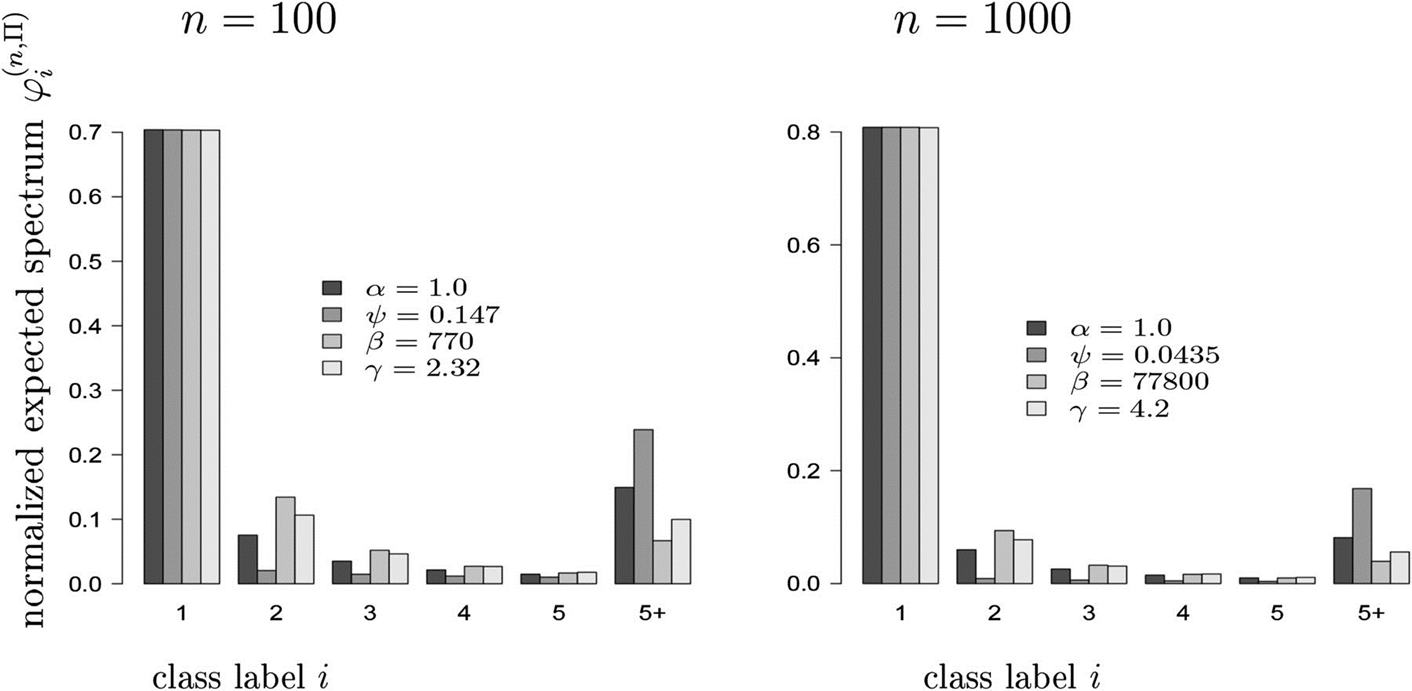
\includegraphics[width=\linewidth]{example-figure}
%%\caption{Example movie (the figure file above is used as a placeholder for this example). \textit{GENETICS} supports video and movie files that can be linked from any portion of the article - including the abstract. Acceptable formats include .asf, avi, .wav, and all types of Windows Media files.
%%}%
%%\label{video:spectrum}
%\end{figure}

\subsection{Sample table}

Table \ref{tab:shape-functions} shows an example table. Avoid shading, color type, line drawings, graphics, or other illustrations within tables. Use tables for data only; present drawings, graphics, and illustrations as separate figures. Histograms should not be used to present data that can be captured easily in text or small tables, as they take up much more space.

Tables numbers are given in Arabic numerals. Tables should not be numbered 1A, 1B, etc., but if necessary, interior parts of the table can be labeled A, B, etc. for easy reference in the text.

\begin{table*}[p]
\centering
\caption{Students and their grades}
\begin{tableminipage}{\textwidth}
\begin{tabularx}{\textwidth}{@{}XXXX@{}}
\hline
{\bf Student} & {\bf Grade}\footnote{This is an example of a footnote in a table. Lowercase, superscript italic letters (a, b, c, etc.) are used by default. You can also use *, **, and *** to indicate conventional levels of statistical significance, explained below the table.} & {\bf Rank} & {\bf Notes} \\
\hline
Alice & 82\% & 1 & Performed very well.\\
Bob & 65\% & 3 & Not up to his usual standard.\\
Charlie & 73\% & 2 & A good attempt.\\
\hline
\end{tabularx}
  \label{tab:shape-functions}
\end{tableminipage}
\end{table*}

\section{Sample equation}

Let $X_1, X_2, \ldots, X_n$ be a sequence of independent and identically distributed random variables with $\text{E}[X_i] = \mu$ and $\text{Var}[X_i] = \sigma^2 < \infty$, and let
\begin{equation}
S_n = \frac{X_1 + X_2 + \cdots + X_n}{n}
      = \frac{1}{n}\sum_{i}^{n} X_i
\label{eq:refname1}
\end{equation}
denote their mean. Then as $n$ approaches infinity, the random variables $\sqrt{n}(S_n - \mu)$ converge in distribution to a normal $\mathcal{N}(0, \sigma^2)$.

\section{Data availability}

The inclusion of a Data Availability Statement is a requirement for articles published in GENETICS. Data Availability Statements provide a standardized format for readers to understand the availability of data underlying the research results described in the article. The statement may refer to original data generated in the course of the study or to third-party data analyzed in the article. The statement should describe and provide means of access, where possible, by linking to the data or providing the required unique identifier.

For example: Strains and plasmids are available upon request. File S1 contains detailed descriptions of all supplemental files. File S2 contains SNP ID numbers and locations. File S3 contains genotypes for each individual. Sequence data are available at GenBank and the accession numbers are listed in File S3. Gene expression data are available at GEO with the accession number: GDS1234. Code used to generate the simulated data can be found at \url{https://figshare.org/record/123456}.

\section{Acknowledgments}
Acknowledgments should be included here.

\section{Funding}
Funding, including Funder Names and Grant numbers should be included here.

\section{Conflicts of interest}
Please either state that you have no conflicts of interest, or list relevant information here.  This would cover any situations that might raise any questions of bias in your work and in your article’s conclusions, implications, or opinions. Please see \url{https://academic.oup.com/journals/pages/authors/authors_faqs/conflicts_of_interest}.

\end{document} 